\documentclass[12pt]{article}

% Packages
\usepackage[margin=1in]{geometry}
\usepackage{setspace}
\usepackage{graphicx}
\usepackage{amsmath, amssymb}
\usepackage{hyperref}
\usepackage{titlesec}
\usepackage{mdframed}
\usepackage{xcolor}
\usepackage{float}


% Spacing
\setstretch{1.2}

\usepackage{xcolor}
\usepackage{hyperref}

\hypersetup{
    colorlinks=true,
    linkcolor=blue,
    urlcolor=blue,
    citecolor=blue
}

\let\oldhref\href
\renewcommand{\href}[2]{\oldhref{#1}{\underline{#2}}}

% Section formatting
\titleformat{\section}{\large\bfseries}{\thesection}{1em}{}
\titleformat{\subsection}{\normalsize\bfseries}{\thesubsection}{1em}{}

% Title info
\title{\textbf{Analysis of Presidential Addresses}}
\author{Madison Byrd \\
Trusted AI\\
}
\date{\today}

\begin{document}

\maketitle
\newpage

\section{Report}

This project was to conduct analysis of inaugural addresses of presidents throughout American history.
These included sentiment analysis and word clouds. These presidents were:
\begin{itemize}
    \item Thomas Jefferson (1801)
    \item Abraham Lincoln (1861)
    \item Woodrow Wilson (1913)
    \item Harry Truman (1949)
    \item Ronald Reagan (1981)
\end{itemize}

The models used to analyze these addresses were VADER and TextBlob, two text analysis models:

\begin{figure}[H]
    \centering
    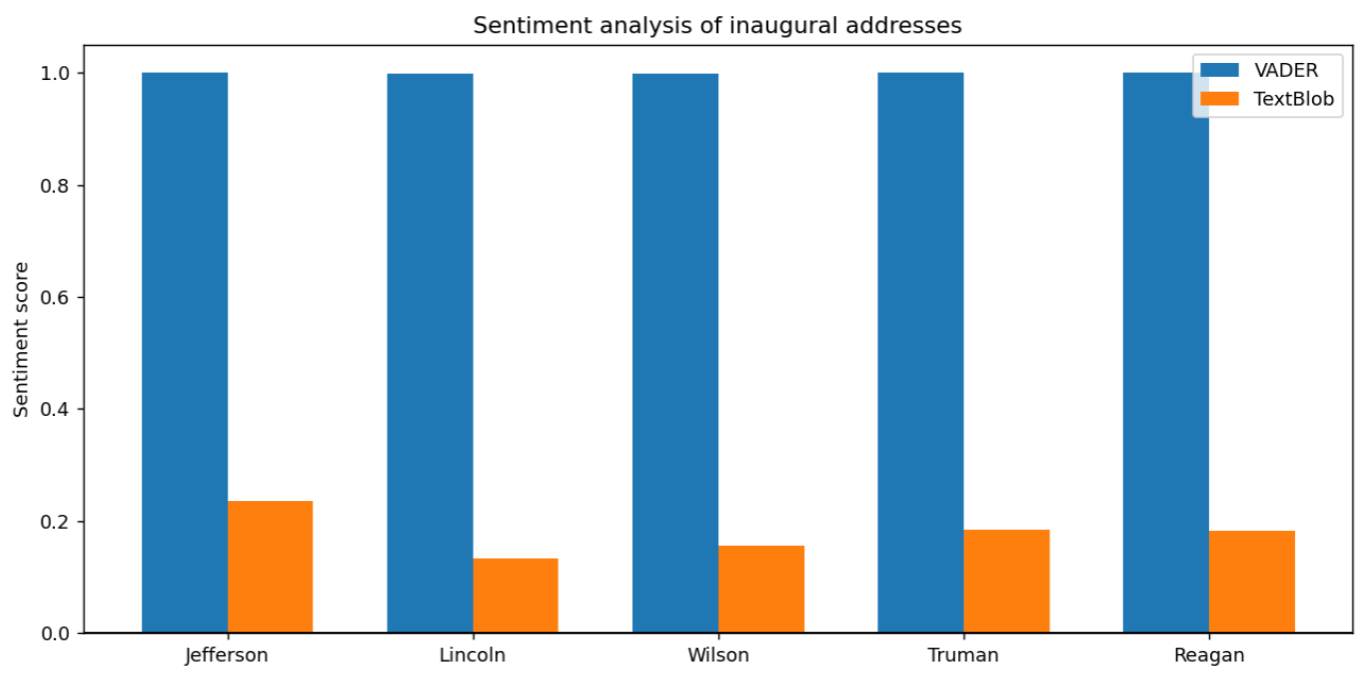
\includegraphics[width=1\textwidth]{sentiment.png}
    \caption{Sentiment analysis by presidential address}
\end{figure}

For sentiment analysis, the results were all very similar for both models (quite positive with VADER
and somewhat positive with TextBlob, probably because presidents use similar rhetoric
and want their speeches to sound positive. TextBlob's metrics were more varied than VADER's and showed
Lincoln as having the least positive sentiment. This makes sense because Lincoln's address was given near the beginning
of the American Civil War.
Of the word clouds, my favorite was Truman's:

\begin{figure}[H]
    \centering
    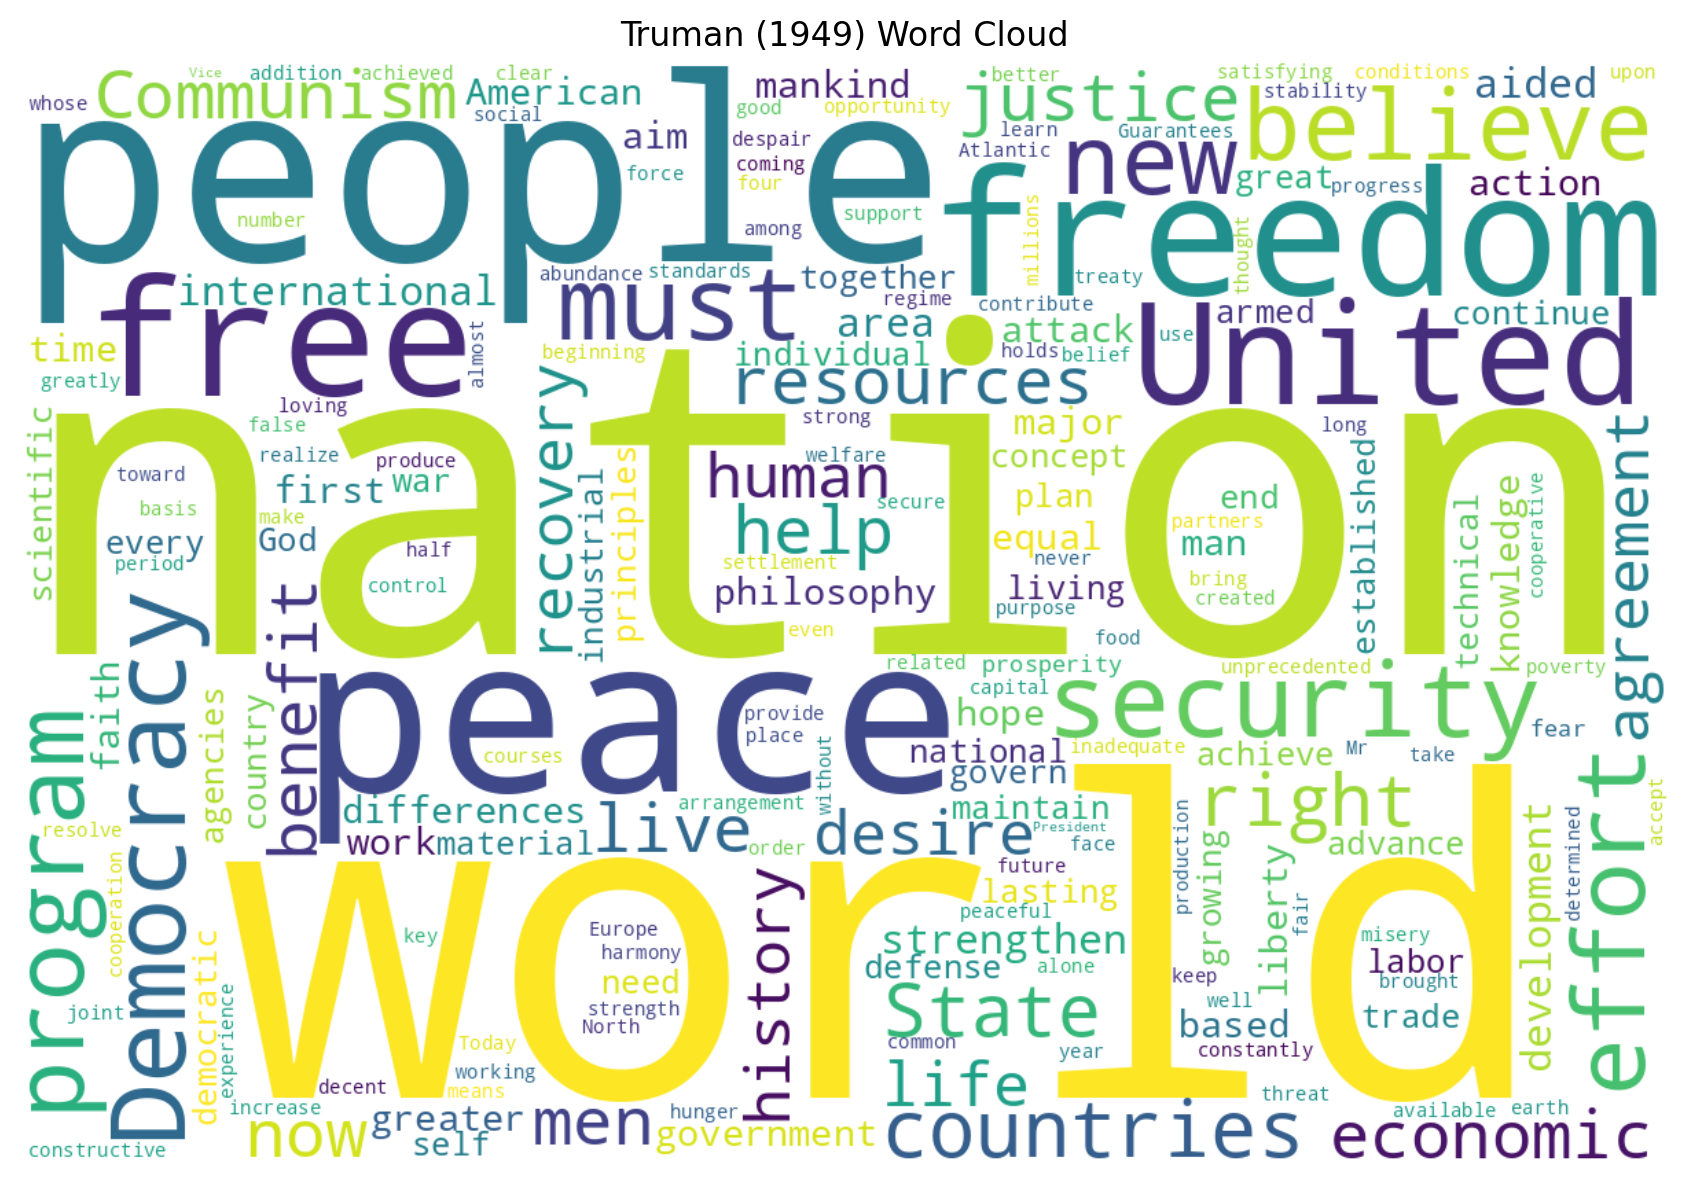
\includegraphics[width=1\textwidth]{../inaugural_wordclouds/truman_1949.png}
    \caption{Truman's word cloud}
\end{figure}

This one makes sense because in 1949 WWII had just ended and the United States was the only major power
left relatively intact, and the United Nations was forming to prevent another world war. As such, 
words like "world", "peace", and "people" are very prominent.



\end{document}
